\begin{frame} \frametitle{Problem setup: We model the ultrasound-alveolar interaction as a 2D, compressible, inviscid fluid system.}
  \begin{figure}
    \centering
    \def\svgwidth{0.48\textwidth}
    {\footnotesize
      \import{../figs/lung_figs/}{usbe_lung_schematic2.pdf_tex} \hfill%
    }
    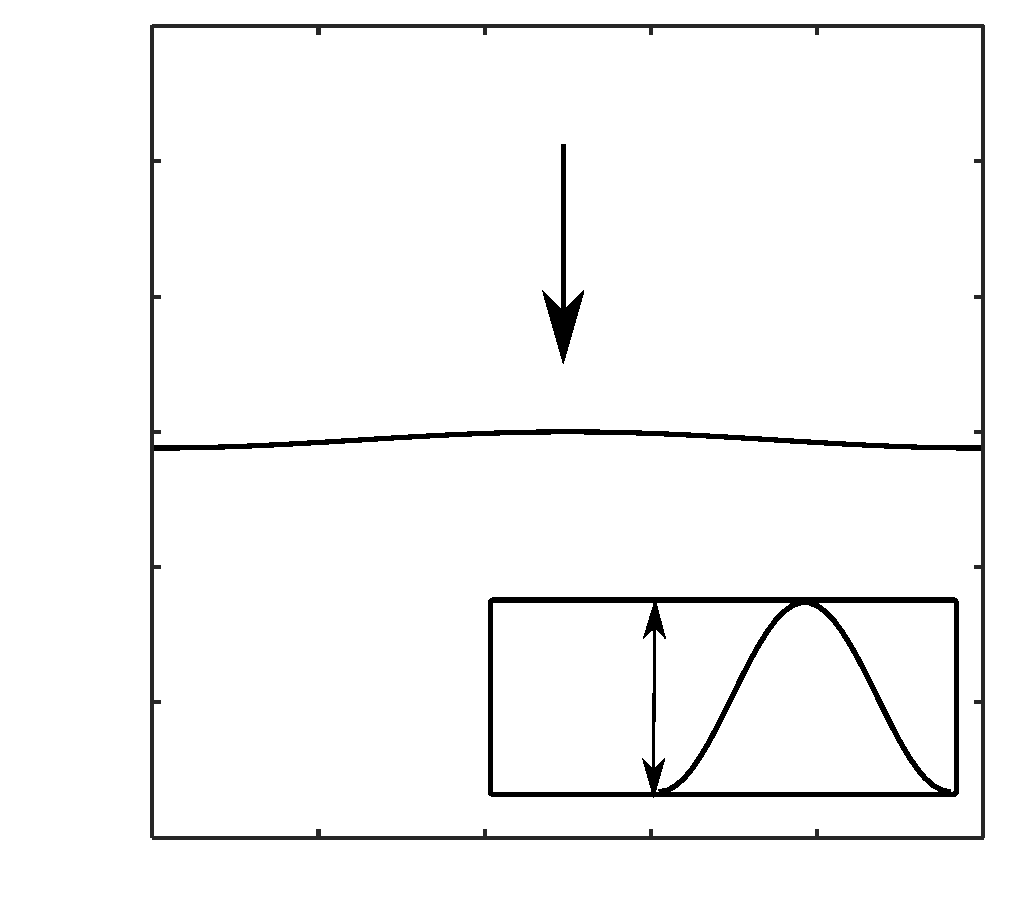
\includegraphics[width=0.48\textwidth]{../figs/lung_figs/usbe_model_schematic} \hfill
  \end{figure}
  An acoustic wave impinges downward from water toward a perturbed air interface $(a_0\equals0.06\lambda)$.
  \note{
    \begin{enumerate}
    \item We model an acoustic wave impinging downward from tissue (liquid) onto an air inside an alveolus.
    \item We use an initially sinusoidal interface with a wavelength $\lambda$, which is the width of our domain. 
    \item And a peak-to-peak perturbation amplitude of $0.06\lambda$
    \end{enumerate}
    }
\end{frame}
%%% Local Variables:
%%% mode: latex
%%% TeX-master: "../main"
%%% End:
